%%%%%%%%%%%%%%%%%%%%%%%%%%%%%%%%%%%%%%%%%%%%%%%%%%%%%%%%%%%%%%%%%%%%%%%%%%%%%%%%
\chapter{Automatic Activity Generation Implementation}\label{sec:impl}

\begin{chapterBody}

\begin{figure}[ht]
    \centering
    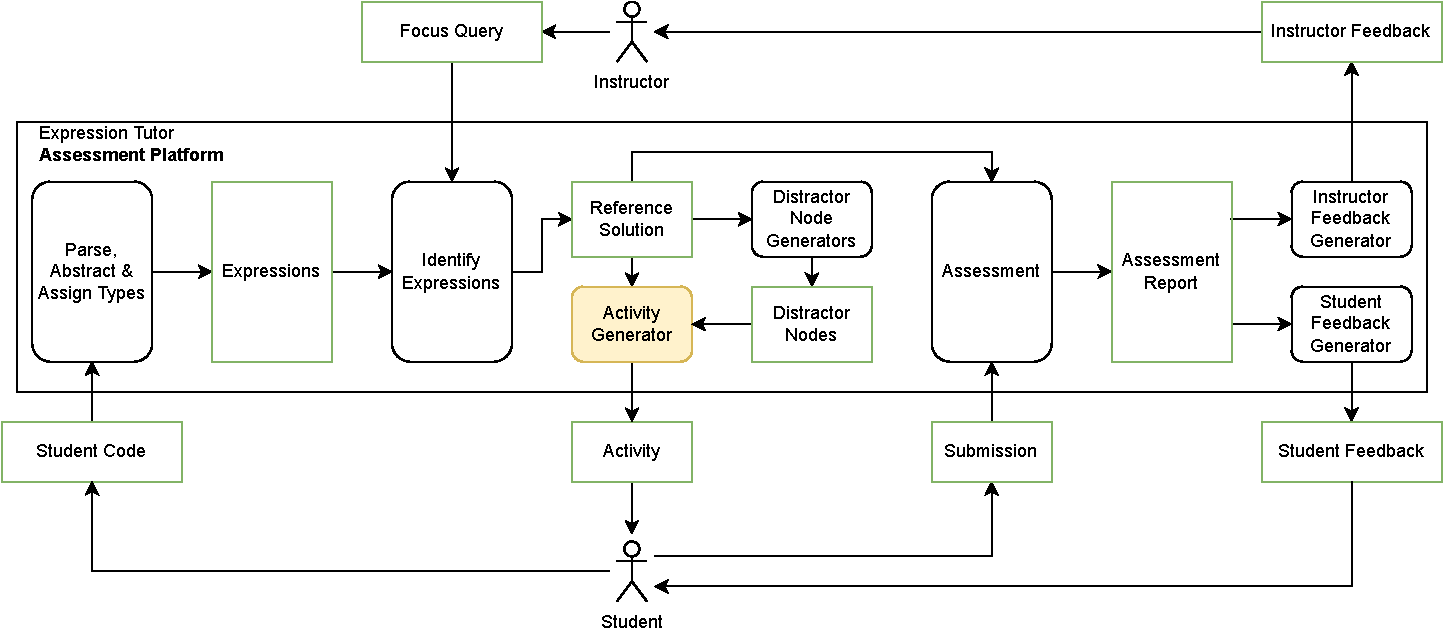
\includegraphics[width=\textwidth]{res/6/et_loop_ag.pdf}
    \caption{Generating activities by using a reference solution and
distractor nodes.}
    \label{fig:ag-intro-loop}
\end{figure}

In this chapter we combine the contributions described and implemented in the
three prior chapters into a system that can be used for automated generation and 
assessment of the personalized activities.

The implementation makes use of the infrastructure provided by GitHub (such
as GitHub Actions and GitHub Classroom). Instructors create programming
assignments in a template Git repository. This repository is then used by
GitHub Classroom to create a Git repository for each student. The students then
pushes their submission to their Git repository.

The system then uses GitHub Actions to automatically analyze each
students' code \hfill\break (\textbf{Section~\ref{sec:impl-aag}}) and it
generates a GitHub Issue with a link to an Expression Tutor activity.
In that activity, the student needs to explain an expression selected from their
submitted code.
The expressions are selected automatically based on a focus query provided by
the instructor (Chapter~\ref{sec:etl}).
This means that each student gets to explain an expression from their own code
but the expressions are all about a concept chosen by the instructor.

The system then catalogues all of the students' submissions into
activity groups \hfill\break (\textbf{Section~\ref{sec:impl-agi-ag}}).
Then, Instructors 
(\textbf{Section~\ref{sec:impl-agi-instructors}}) can then visualize the
submissions on the Expression Tutor platform.

\section{Automatic Activity Generation}\label{sec:impl-aag}

The activity generation process can be formally defined as a
function that takes an expression tree diagram of the reference
solution and a set of distractor nodes and produces an activity, as
highlighted in \textbf{Figure~\ref{fig:ag-intro-loop}}.

\[
\text{activityGeneration}:
\left(\text{ExprTreeDiagram}, \text{Set}\left[\text{Node}\right]\right)
\rightarrow
\text{Activity}
\]

The main challenge that we need to overcome to accomplish automatic
activity generation is to perform an analysis of the student's code to
select and extract expressions.
The analysis of code–bases consisting of multiple files requires the
analyzed code to be in a file–system that is readable by the program performing
the analysis. This limitation comes from the type–resolution step of the
analysis. It requires looking up code defined in different files that may
reside in specific paths to allow the tool to properly type all the
sub–expressions of the Expression Trees.
Another limitation resides in the fact that, due to regulations, sharing
students' code to a third party platform for processing might not be feasible.

To overcome these issues, we package a tool able to analyze source code,
extract and select expressions for a given Expression Tree Language query
(Chapter~\ref{sec:etl}). The output of this process is one or more specifications
that define how to build an Expression Tutor activity. This is defined in
Section~\ref{sec:impl-aag-pkg} and can be represented as a function that takes
a code–base and produces a number of Expression Tutor activities specifications.
The output is a specification file rather than an actual Expression Tutor
activity so that we avoid a circular dependency
(Section~\ref{sec:bg-rw-le-et}).

Further automation is then built upon the output, so that Activities on the
Expression Tutor platform can actually be generated and sent to students.
This is described in Section~\ref{sec:impl-aag-gh}.

\subsection{Packaging Expression Extraction Functionality}\label{sec:impl-aag-pkg}

To provide a simple way to make use of the Expression Tree generation
from source code functionality, we need to package a tool that may be
executed while having access to the file system in which student's source code
is located.

We take advantage of the already highly modular architecture of the
Expression Service (as represented in Figure~\ref{fig:bg-es-arch}), and
select only the modules that are strictly necessary for \textit{expression
sourcing}. This means that the tool is built using only 13 out of the 41 modules
(not counting external dependencies). This reduction in number of included
modules also reduces the final binary size roughly by 60\% (about 23MB for the
minimized binary compared to 57MB for the full binary).
\textbf{Figure~\ref{fig:impl-di-modules}} illustrates the dependency graph
of the expression sourcing feature as opposed to the complete Expression Service
seen in Figure~\ref{fig:bg-es-arch}.

\begin{figure}[ht]
    \centering
    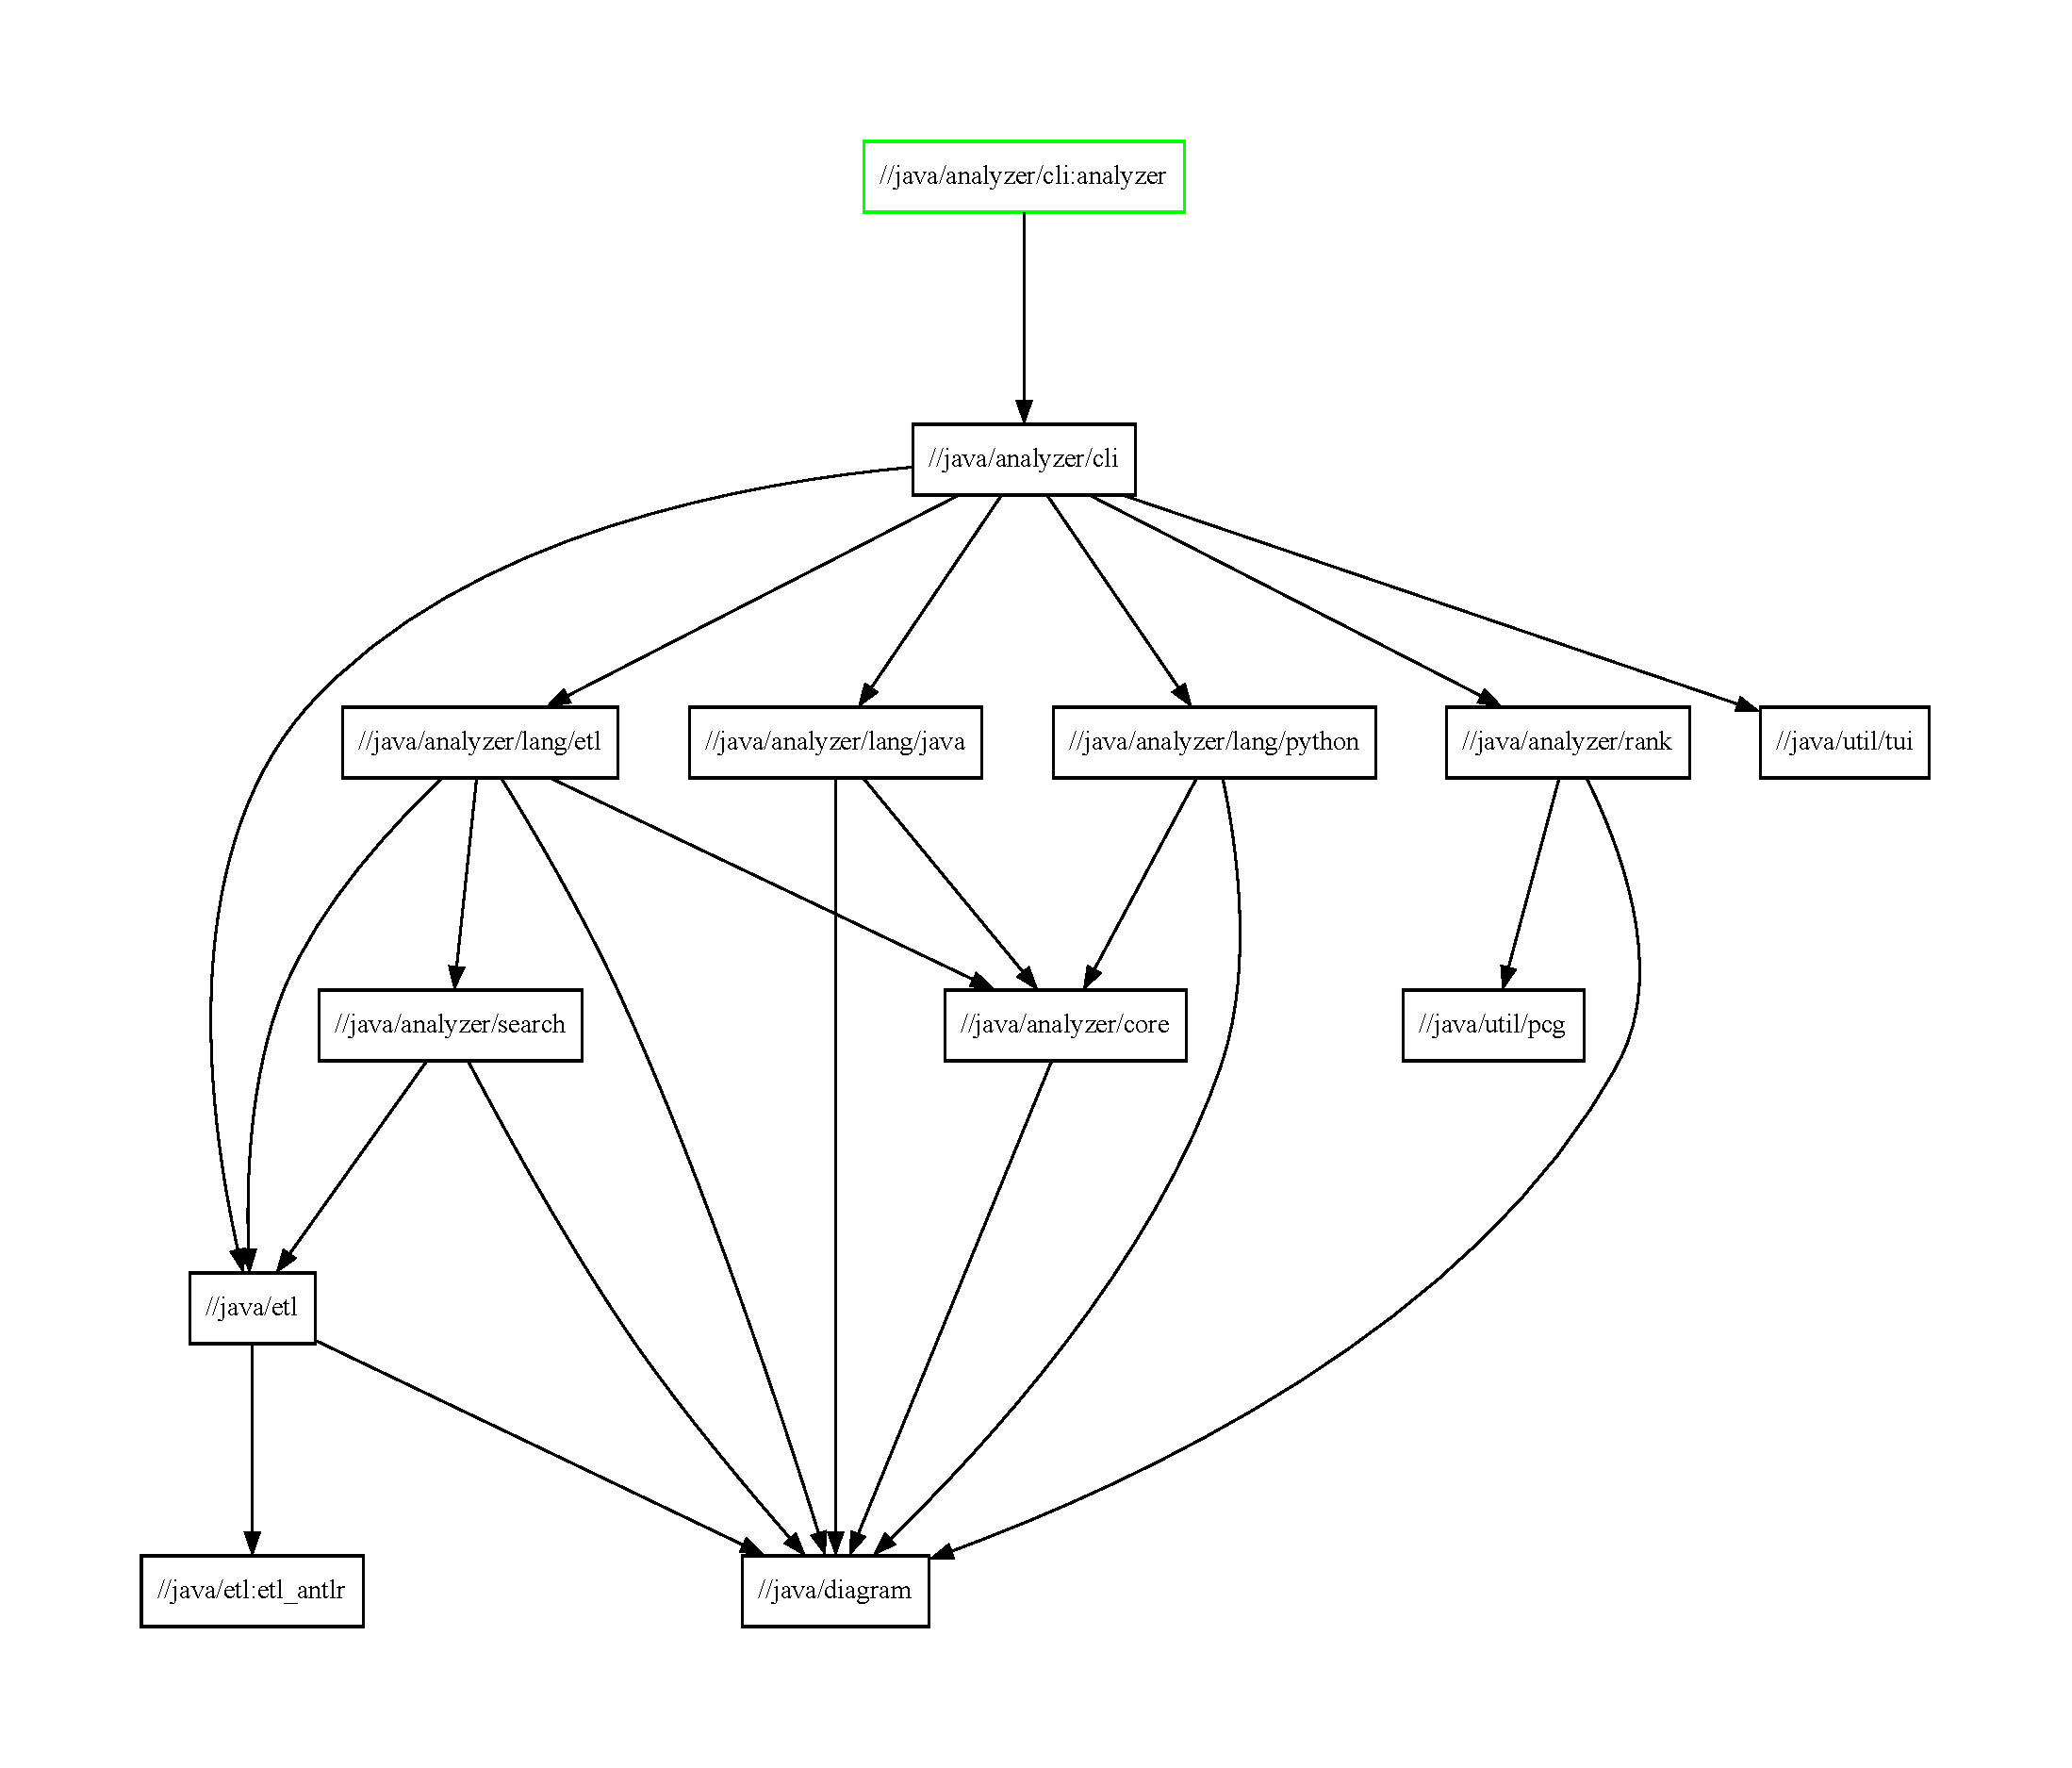
\includegraphics[width=0.6\linewidth]{res/6/expr_serv_analyzer_dep_graph.pdf}
    \caption{Subset of Expression Service modules necessary for expression
sourcing.}
    \label{fig:impl-di-modules}
\end{figure}

For a simplified delivery and execution of the tool, we package it into
a Docker image~\cite{docker_inc_docker_2022}. A Docker image is a template that
can be instantiated to a Docker container, a virtualized environment in which
programs can be executed in a \textit{isolated and standardized} way across
different machines.
The \textit{parent} image being used is \texttt{eclipse-temurin:17-jre} as it
provides a Linux–based Java 17 run–time environment for Expression Service to
be executed.

The minimized version of Expression Service is installed in the
\texttt{/opt/expression-service} path, from which it can be invoked as a
\textit{fat Jar} executable (a Java archive that bundles the main program code 
and all of its dependencies into a single file) by running the command
\texttt{java -jar /opt/expression-service/app.jar}.
By using the Docker volumes functionality, we mount directories from the host
file–system inside the docker image to make those the student's code accessible
to the Expression Service executable to generate Expression Tutor activities.

Since this image only contains Expression Service, and since \textit{Service}
has no dependency on Expression Tutor to avoid circular dependencies between
the Service and Tutor (as described in Section~\ref{sec:bg-rw-le-et}), this
image only generates one Expression Tutor Aativity specification file for each
selected expression.
These files can be supplied as they are to the Expression Tutor API to actually
create an Expression Tutor activity.
An Expression Tutor activity specification file consists of:

\begin{itemize}
    \item A reference solution, which is the Expression Tree built by the tool 
from the original expression in the source code.
    \item The code snippet of said expression, provided to the student in the
activity directive specifications.
    \item An initial state for the student's submission, as specified in
Chapter~\ref{sec:dn}.
    \item Optionally, an activity group identifier, to group different
activities from different students (Section~\ref{sec:impl-agi-ag}). 
\end{itemize}

\subsection{GitHub Action}\label{sec:impl-aag-gh}

GitHub Classroom is an educational tool for the GitHub platform which allows
instructors to easily create and manage coding assignments for
students~\cite{github_inc_2020_2020}. We want to provide an easy way to easily
integrate Expression Tutor activities into students' assignment workflow.
This is made possible with a GitHub action. These are used to ``automate,
customize, and execute software development workflows right in a GitHub
repository''~\cite{github_inc_github_2023}. One way to build such Actions is to
build a Docker image. Parameters to its execution and environment variables
provide access to the GitHub API and the code in the repository it is being
executed on.

The GitHub action we develop builds upon the Docker image described in
Section~\ref{sec:impl-aag-pkg} and extends it. The code in the repository is
automatically given as input to the Expression Service tool.
A number of expressions, matching a user–supplied query, are selected and
converted into Expression Tutor activity configuration files. These are then
uploaded directly to Expression Tutor. Finally, the student receives a GitHub
issue detailing the instructions to complete the Expression Tutor activity with
contextual information about the expression, as depicted in
\textbf{Figure~\ref{fig:impl-gi-issue}}.

\begin{figure}[ht]
    \centering
    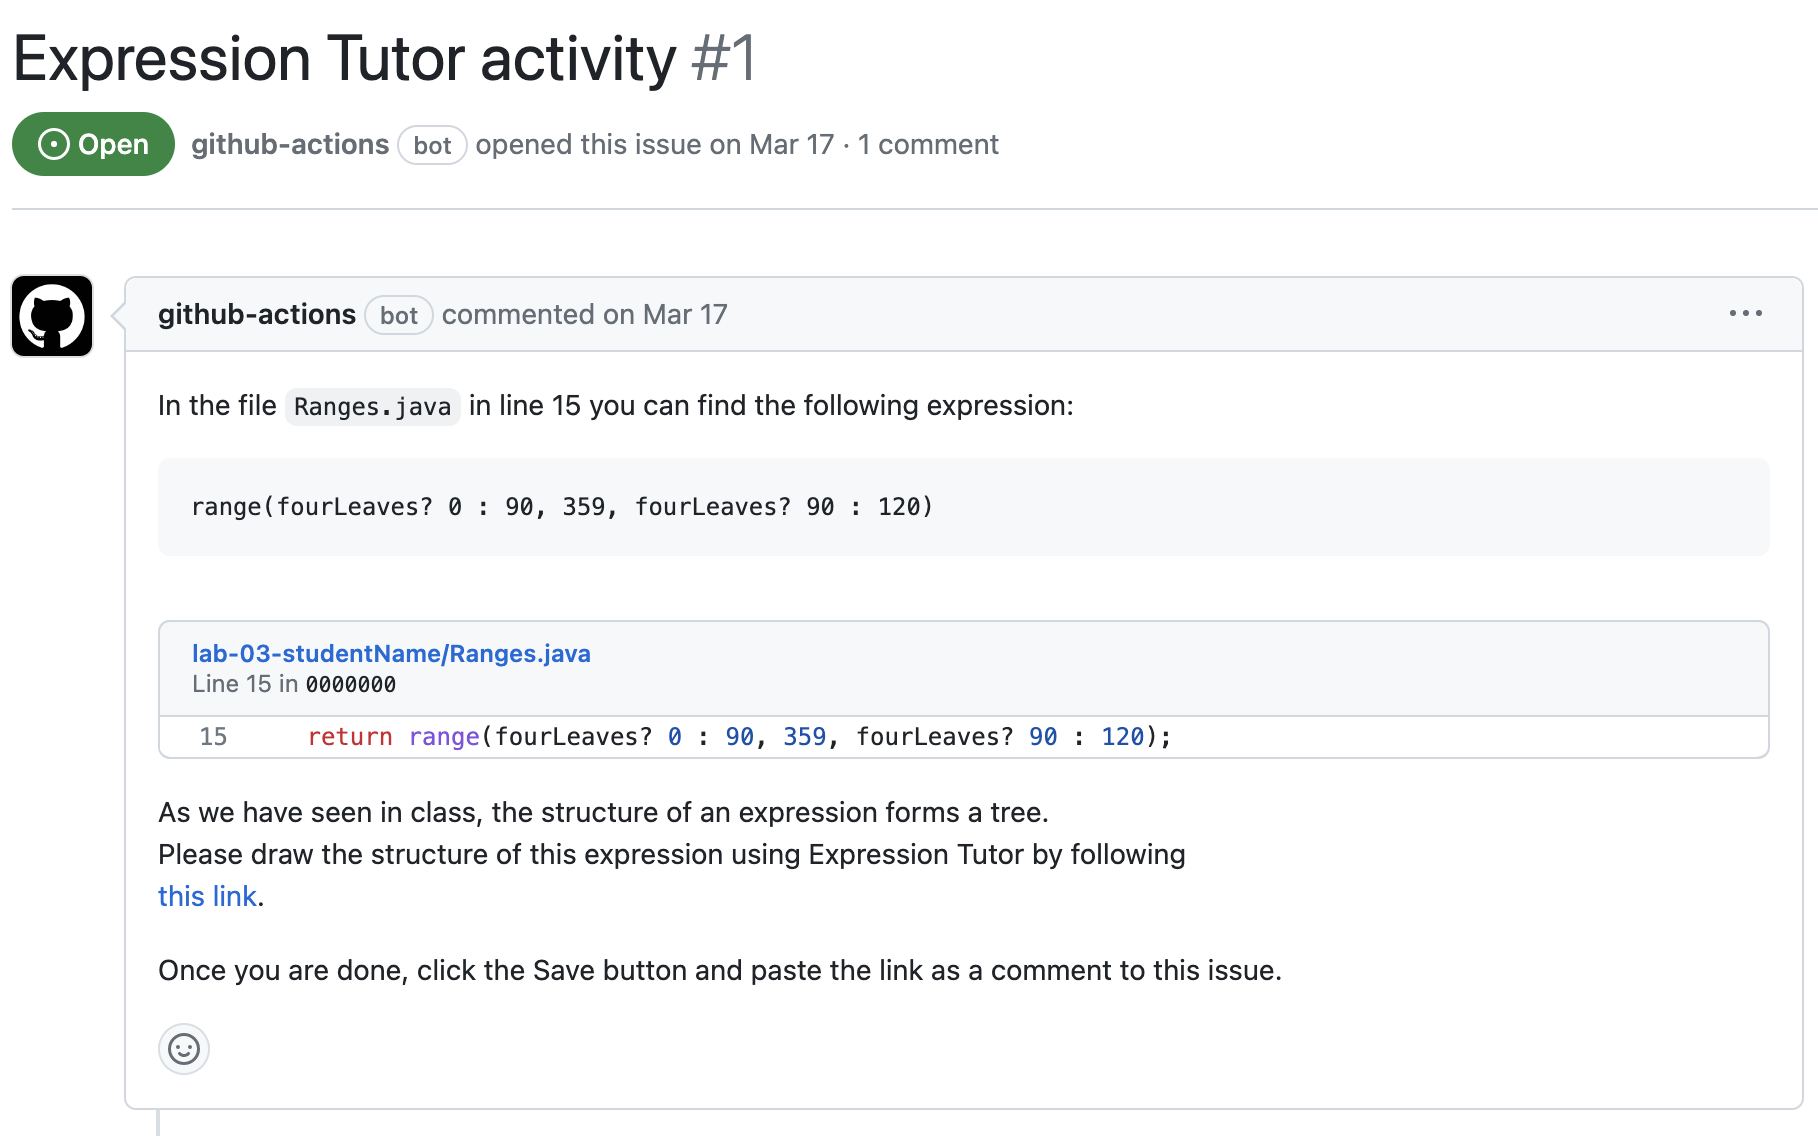
\includegraphics[width=\linewidth]{res/6/gh_activity_issue.png}
    \caption{The student receives an Issue regarding the Expression Tutor 
Activity.}
    \label{fig:impl-gi-issue}
\end{figure}

The GitHub action can be configured by the instructor when creating the
template repository for an assignment. The configuration allows to specify the
following:

\begin{itemize}
    \item The number of expressions to select / activities to generate.
    \item The path of the directory containing the files that are analyzed.
    \item Identifier of the activity group (as defined in
Section~\ref{sec:impl-agi-instructors}) to associate the generated activities to.
    \item Additional files and directories in the repositories to add to
the Java class–path of analyzed files for type resolution.
\end{itemize}

This configuration is to be written in a GitHub action workflow file,
such as the one in \textbf{Listing~\ref{lst:impl-gi-workflow}}.

\subsection{Expression Selection}\label{sec:impl-aag-select}

To prevent different students having the same exercise to solve, we want to
introduce a certain degree of randomness to how the expression for the activity
is selected. Moreover we do not want to use any form of global state to
keep track of other expressions that were used for other activities within the
same activity group.

To achieve this, all expression tree diagrams that matched the query are ranked
and the top $ N $ are selected (where $ N $ is the number defined in the
configuration of the GitHub action as described in
Section~\ref{sec:impl-aag-gh}).

Diagrams are initially ranked by depth into an ordered list in ascending order
(lower depth diagrams appear before higher depth ones).
We define a diagram's depth The maximum depth of all of its nodes.
The depth of a node is the number of edges from said node to the diagram's root
node. A root node (and also a diagram containing only one node) has a depth
of 0. Then, to introduce some controlled randomness into the ranking system to
ensure different expressions are selected for different students, all the
expressions that have depth $ d \mid d < \text{min\_depth} + 2 $ are shuffled at
the beginning of the ranked list.
From this list, the first $ N $ diagrams are taken.

\section{Instructors and Activity Groups on Expression Tutor}\label{sec:impl-agi}

To allow instructors to easily catalogue and visualize the outcomes of the
activities submissions, we introduce the concept of \textit{Instructors}
(Section~\ref{sec:impl-agi-instructors}) and \textit{activity group}s
(Section~\ref{sec:impl-agi-ag}) to the Expression Tutor platform.

\subsection{Instructors}\label{sec:impl-agi-instructors}

The Expression Tutor platform offers a number of features made exclusively for
instructors that should not be accessible by students. One such example would
be the online \textit{expression analyzer} functionality, which allows to
supply source code and generate Expression Trees from expression found within
user–supplied content.
Moreover, with the introduction of new features described in this thesis, such
as Assessment (\textbf{Section~\ref{sec:fb-assess}}) and activity groups
(\textbf{Section~\ref{sec:impl-agi-ag}}), the need to prevent students to access
features that might allow them to \textit{solve} Expression Tutor activities
for them increases.

This can be solved by introducing the concept of instructors on the 
platform. At the same time, while implementing this system, there are a number
of requirements\footnote{The use of``MUST'', ``MUST NOT'', ``REQUIRED'',
``SHALL'', ``SHALL NOT'', ``SHOULD'', ``SHOULD NOT'', ``RECOMMENDED'', ``MAY'',
and ``OPTIONAL'' is per the IETF standard defined in 
RFC2119~\cite{bradner_key_1997}}:

\begin{enumerate}
    \item Instructors–exclusive functionalities SHALL NOT be openly accessible
to any user of the platform. An instructor MUST authenticate themselves on the
platform to enable access to more functionalities that are not intended for
usage by students.
    \item Expression Tutor SHALL NOT request any kind of personal or sensitive
information about any user of the platform.
    \item An instructor MAY sign up on their own, but they MUST be manually
approved by a trusted entity before they are allowed to make use of 
instructor–exclusive functionalities. 
    \item Authentication of instructors MUST be equally implemented on both
the website and the HTTP APIs that are publicly offered.
\end{enumerate}

\subsubsection*{Implementation}

An instructor instance is identified by a unique randomly generated  immutable 
id. Each instructor instance possesses a token, that is used to authenticate API
requests and on the website when making use of instructor–exclusive features
(Requirements~1, 4) (\textbf{Figure~\ref{fig:impl-instructor-token}}). This
token may be re–issued at any time from the instructor themselves from the
instructor profile page (\textbf{Figure~\ref{fig:impl-instructor-profile}}).

\begin{figure}[ht]
    \centering
    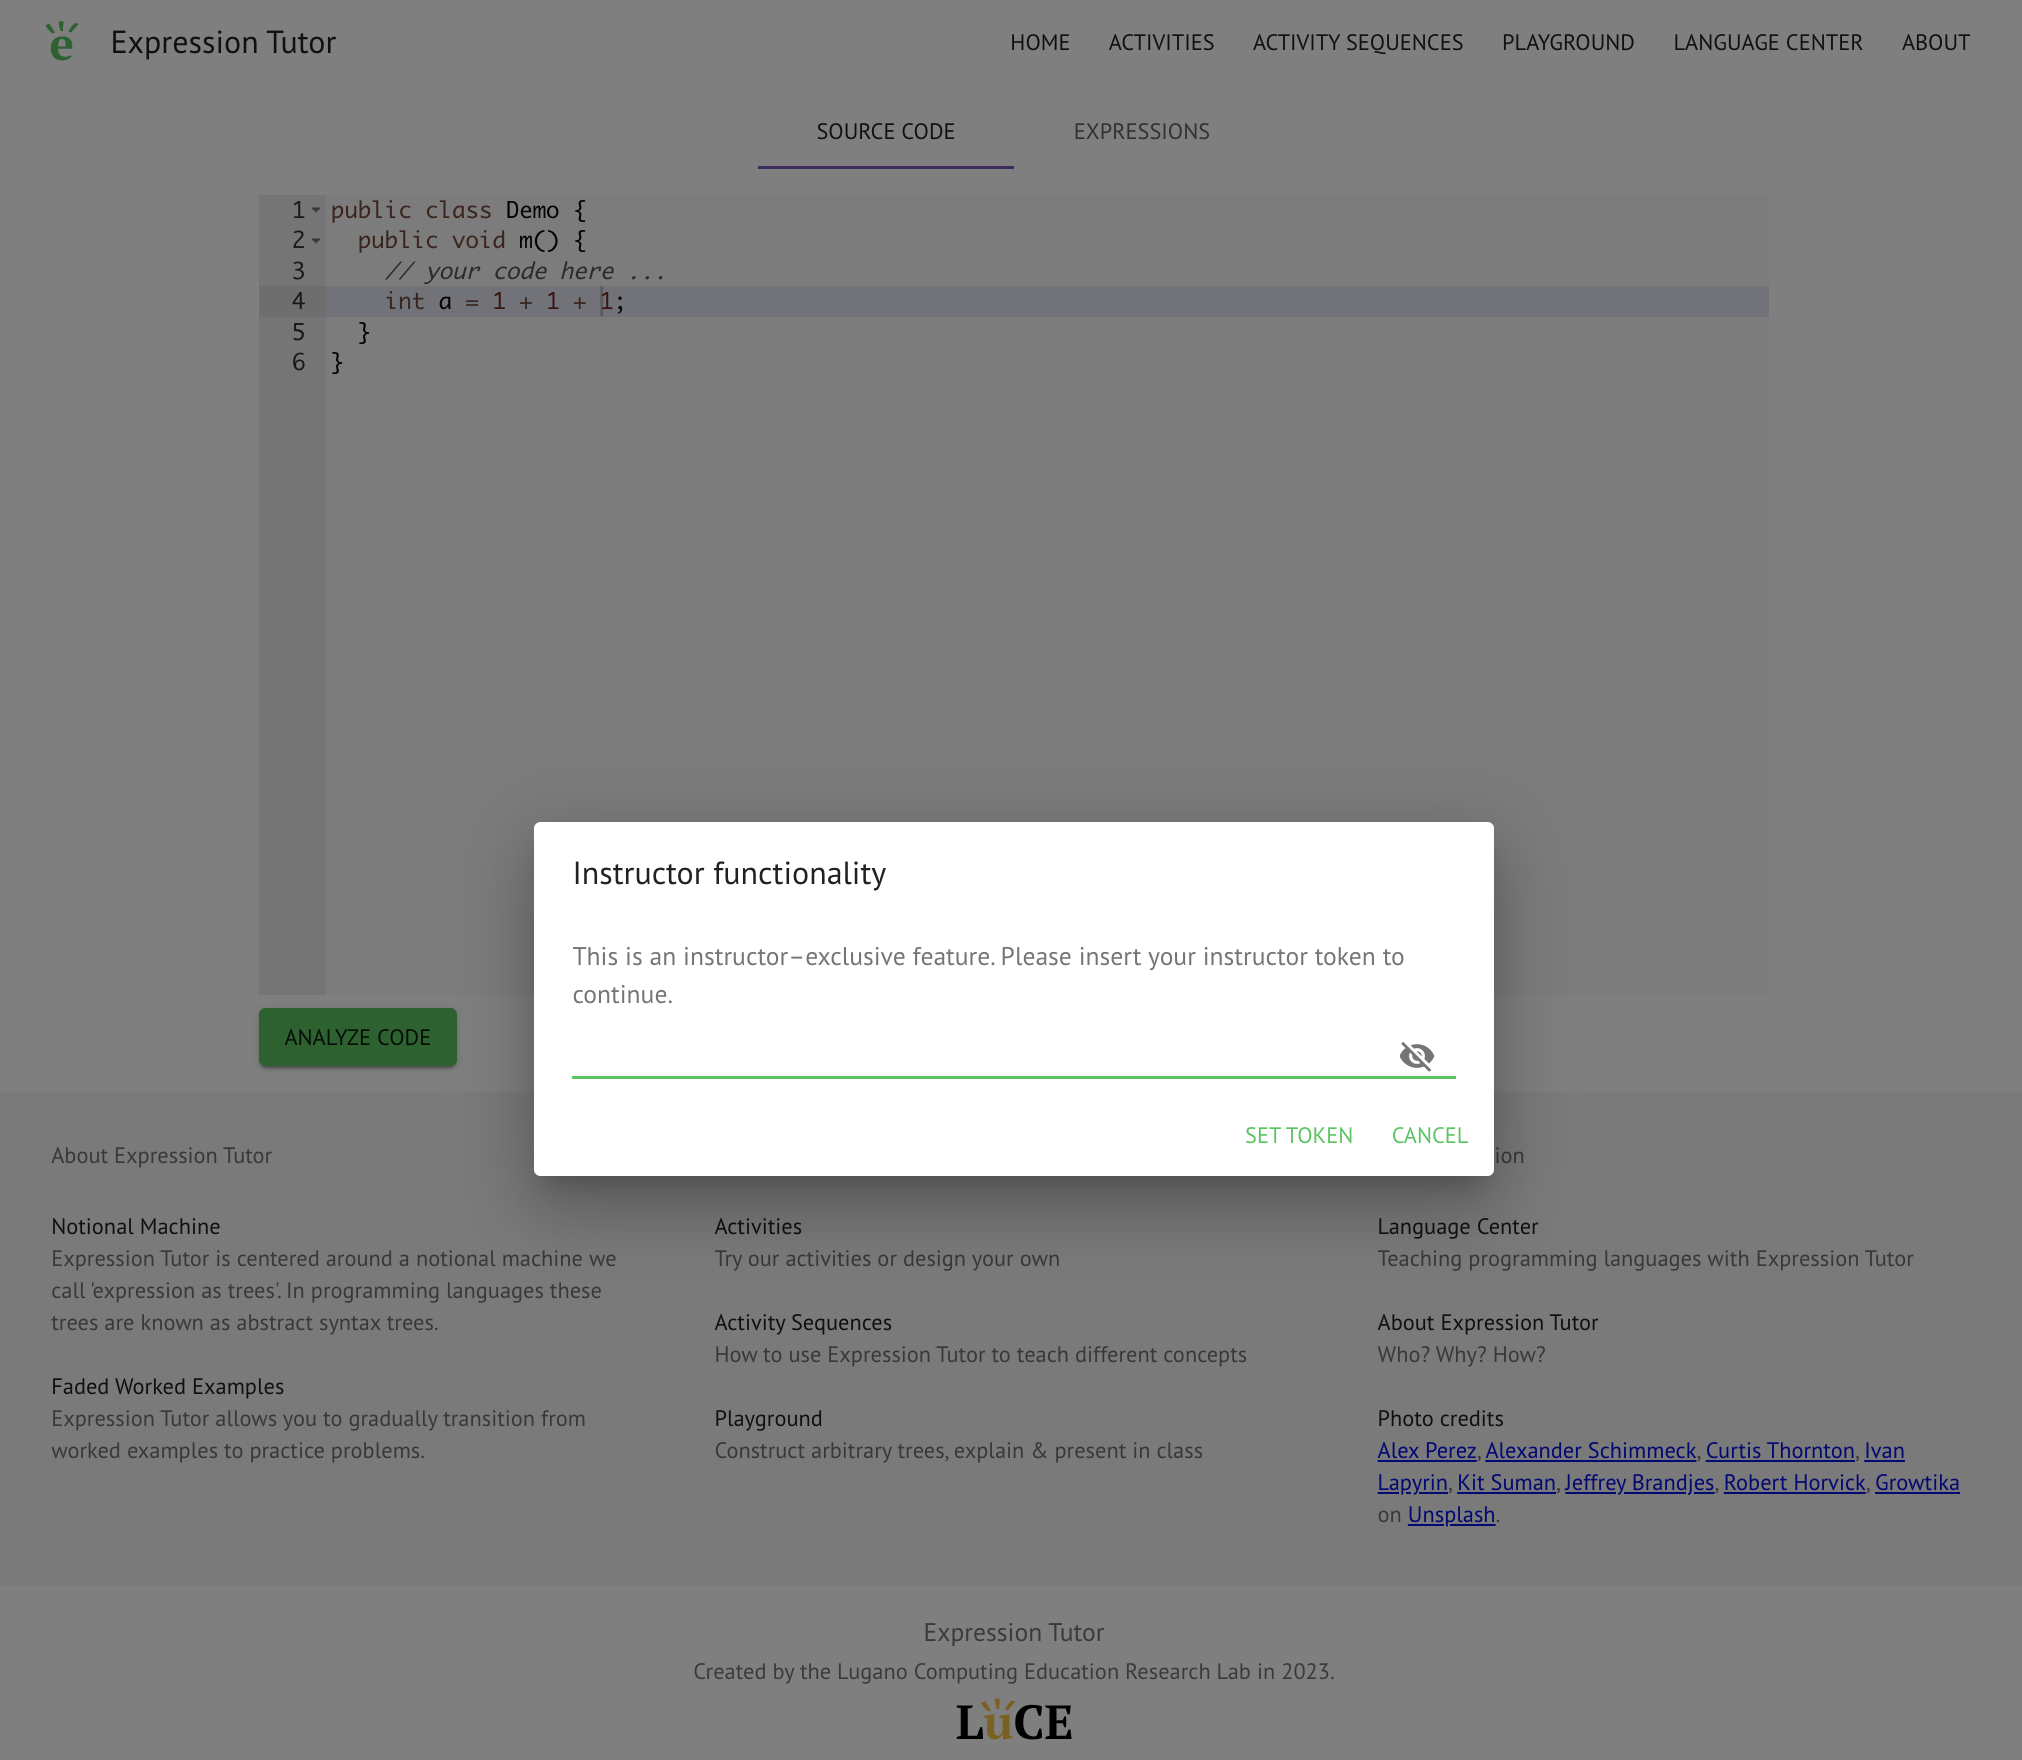
\includegraphics[width=0.8\textwidth]{res/6/instructor_token.png}
    \caption{Instructor token is required to use instructor–exclusive
functionalities such as the online expression analyzer.}
    \label{fig:impl-instructor-token}
\end{figure}

\begin{figure}[ht]
    \centering
    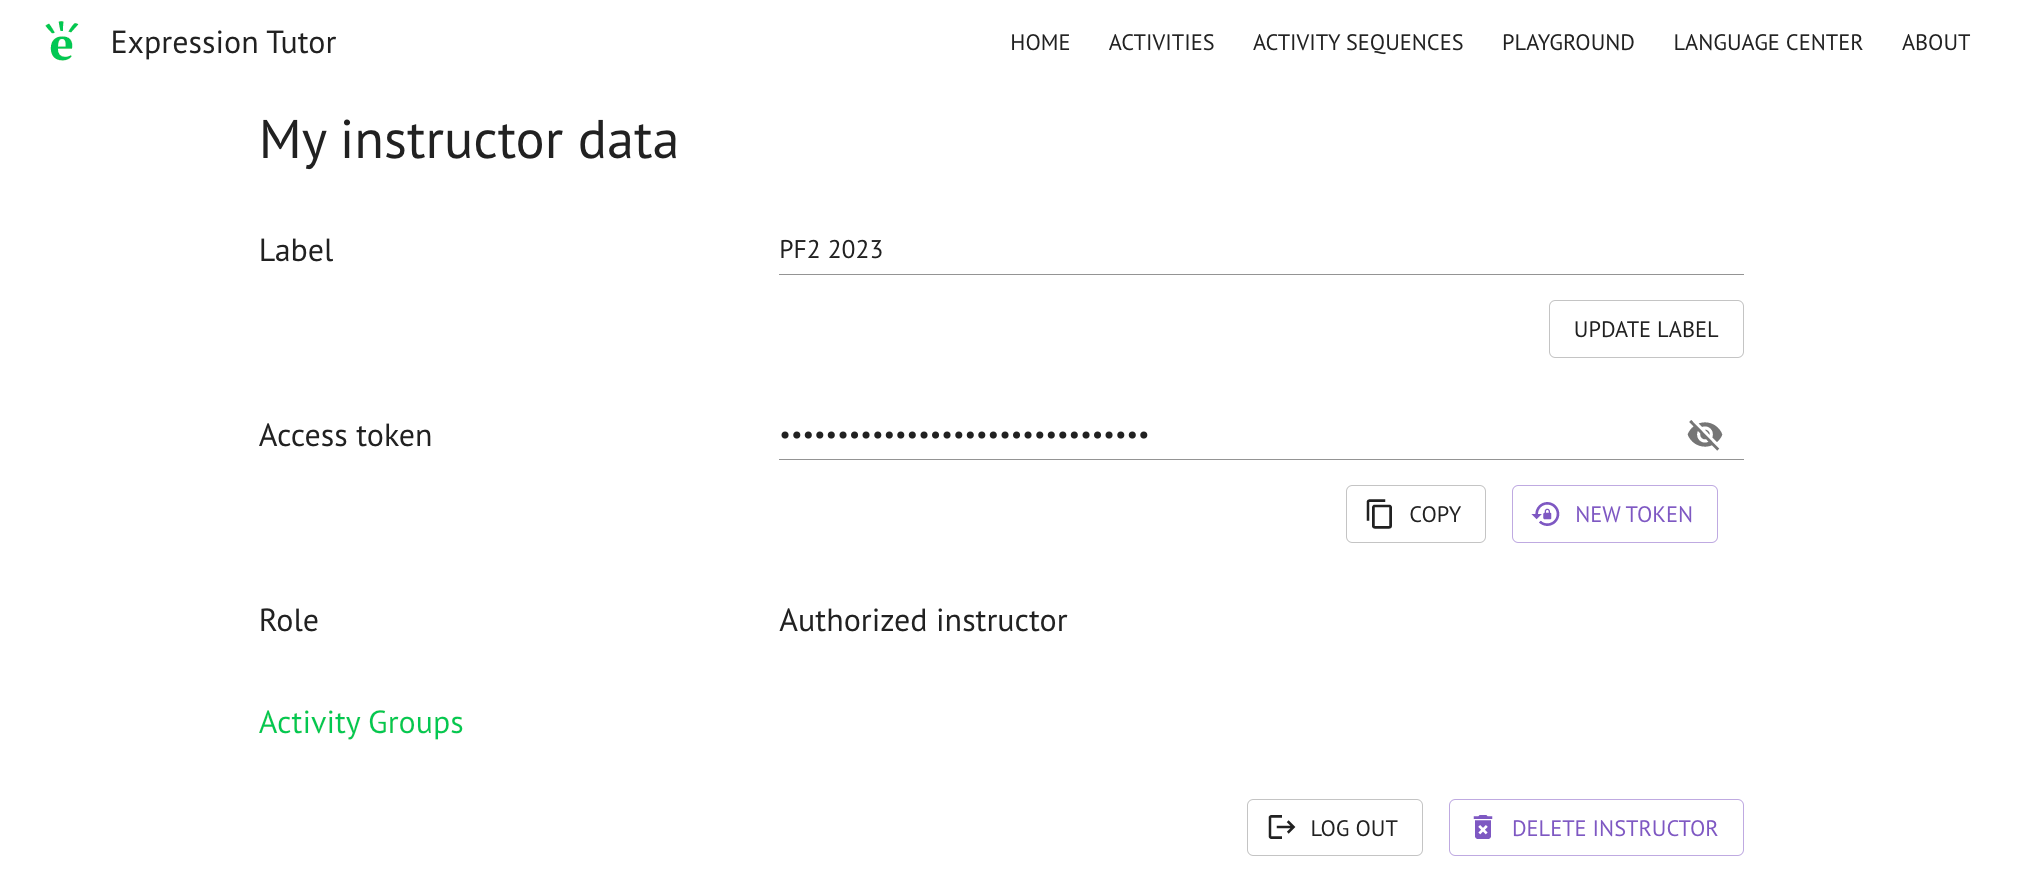
\includegraphics[width=0.8\textwidth]{res/6/instructor_profile.png}
    \caption{Instructor profile page on Expression Tutor.}
    \label{fig:impl-instructor-profile}
\end{figure}

A role is also assigned to Instructors instances. The ``Administrator'' role
allows this instance to create new Instructor instances, change their roles
(which includes approving their access to instructor–exclusive
functionalities), re–issue tokens and delete any existing instructor instances
(\textbf{Figure~\ref{fig:impl-instructor-admin}}).
By default, newly created instructors are assigned the ``Unauthorized'' role,
which effectively restricts them from accessing any instructor–exclusive 
feature.
For that, they must be granted the ``Authorized'' role by an administrator
instructor (Requirement~3).

\begin{figure}
    \centering
    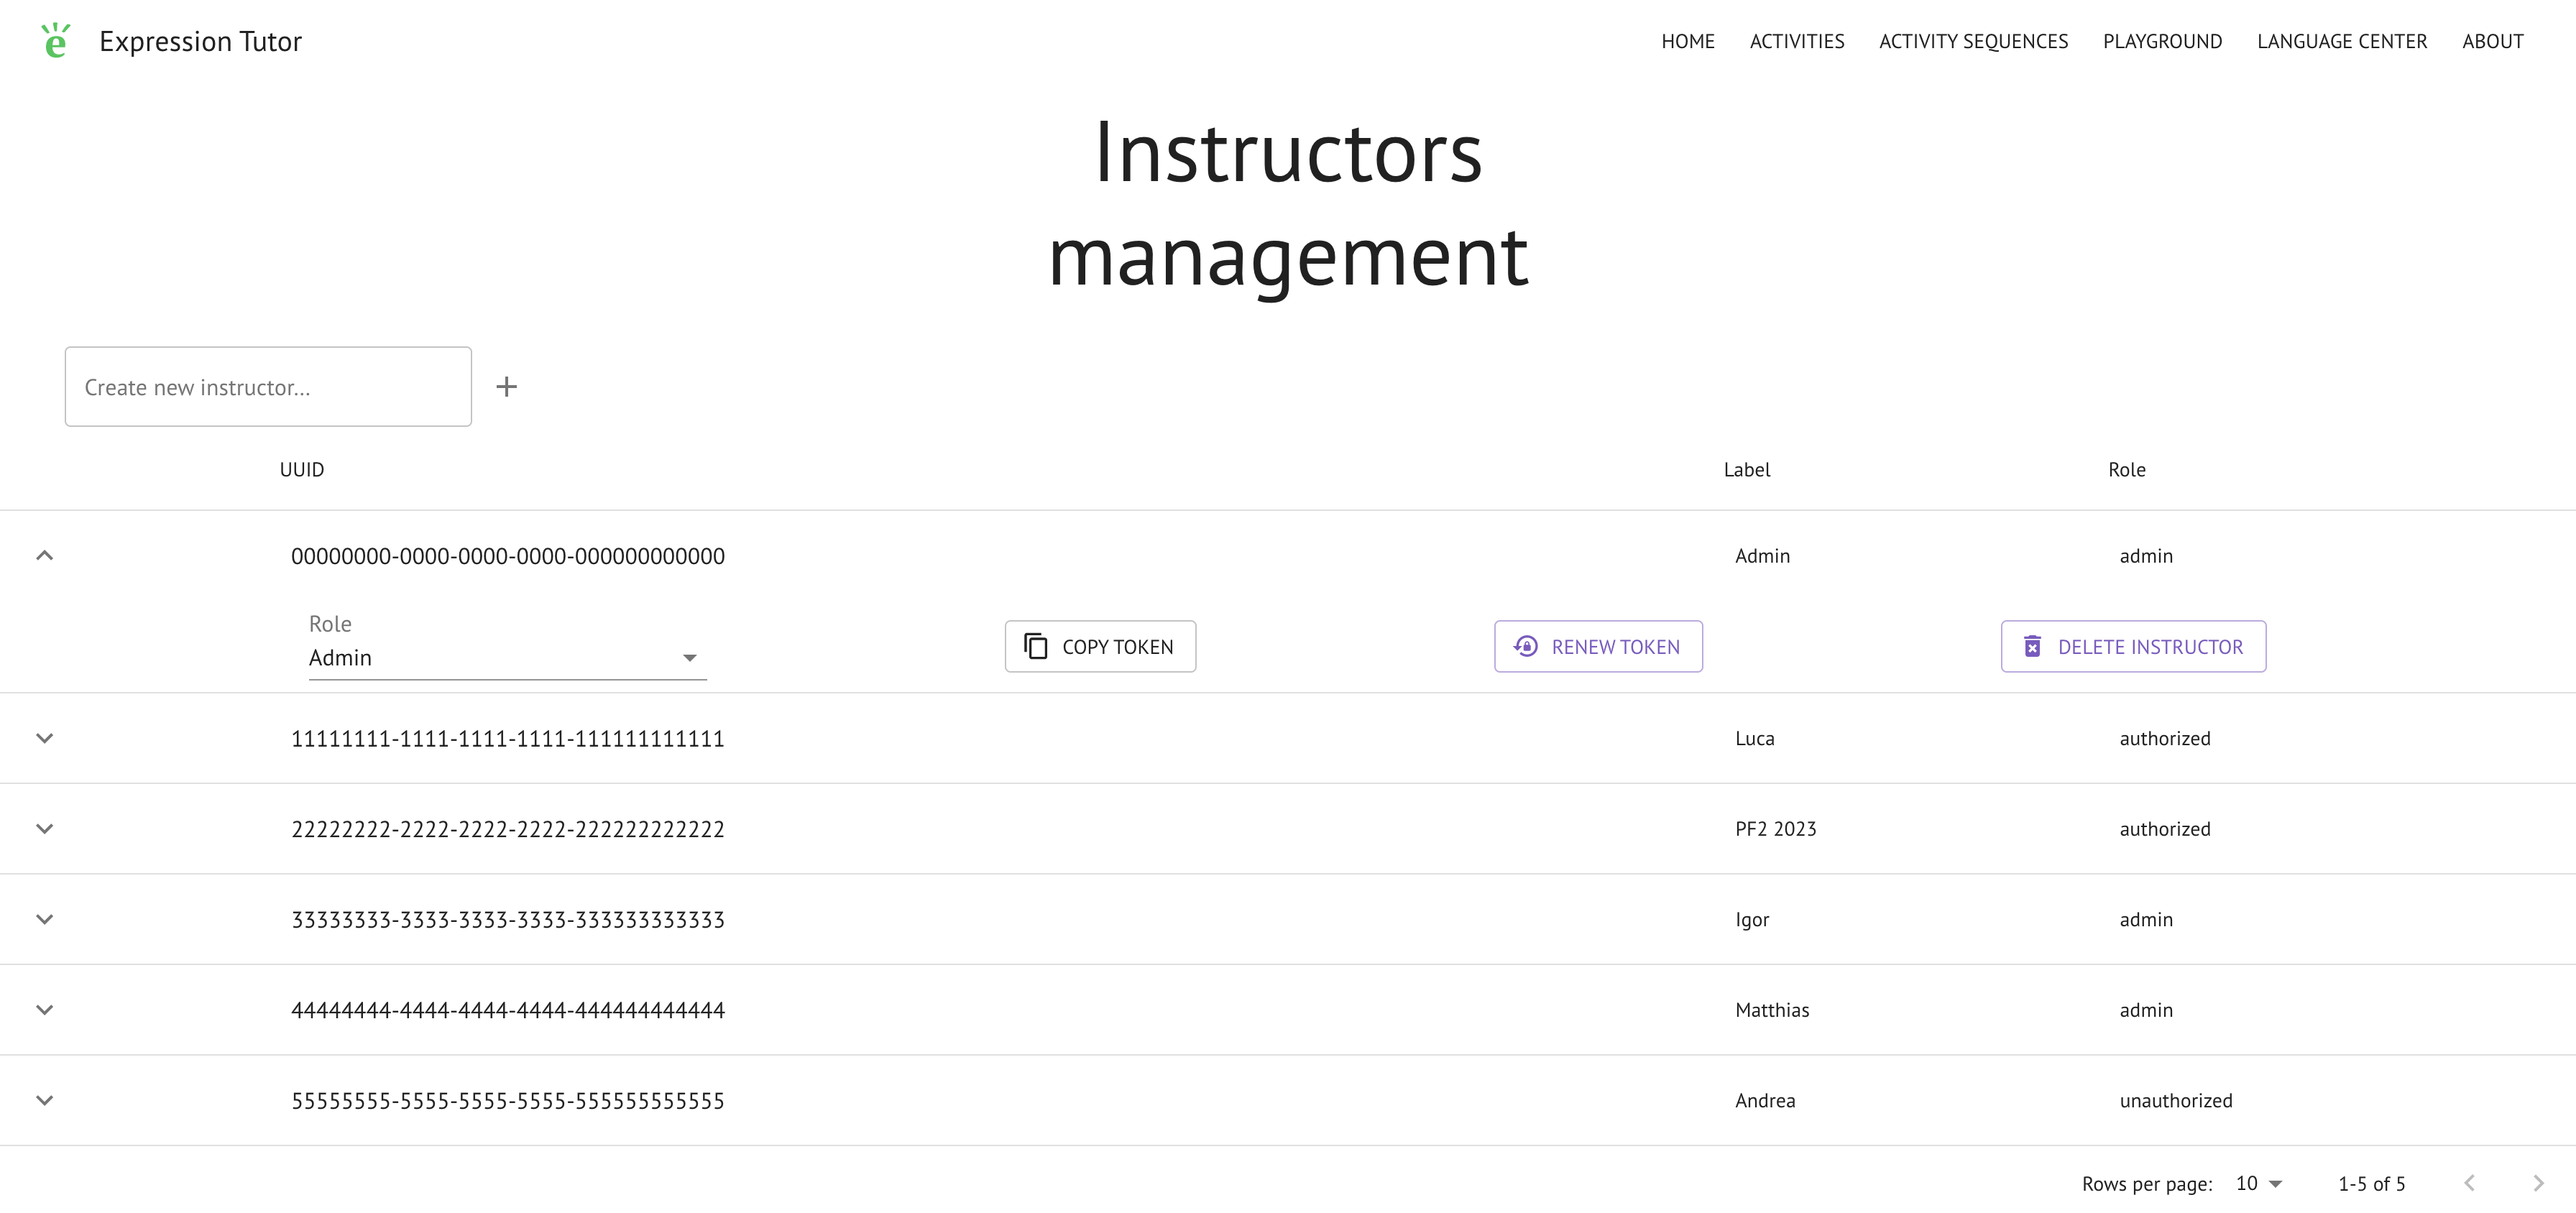
\includegraphics[width=0.8\textwidth]{res/6/instructor_admin.png}
    \caption{Instructors management administrator user interface.}
    \label{fig:impl-instructor-admin}
\end{figure}

Lastly, each Instructor instance allows the owner to define a label that
serves no purpose other than facilitating distinguishing and recognizing
an instructor instance from another. This label has no content requirements,
so that no personal data shall be requested of the instructor to make use of
the platform (Requirement~2). One use case for this label is facilitating
the request to an Administrator to issue a new token for an instructor who
may no longer use the previous one: a user supplied string is easier for
a person rather than the long sequence of randomly–generated characters 
that is the unique id of the Instructor instance.

To create an account instance, one may use the Expression Tutor API
\texttt{POST /api/instructor} and supply a JSON–formatted body
containing a \texttt{label} string attribute. The server shall then reply
with the information about the newly created Instructor instance, including
the token used to be authenticated on the website and the API calls.
Alternatively, an authenticated ``Administrator'' Instructor instance may
create a new instance from the administration dashboard on the Expression
Tutor website.
The \textit{sign–up} process is not locked behind authentication because of the
proverbial ``chicken and egg'' problem. By default, Instructor instances are not
allowed to access any instructor–exclusive feature until they are manually
approved by an administrator. But if there is no administrator instructor 
instance because there existed no other Instructor instances, then there can
not be any instance which is authorized. To solve this problem, the API to sign
up is left open and the very first Instructor instance that is created in
the database, is also automatically given the ``Administrator'' role.

Alternative candidate implementations of this system involved the usage of
the OAUTH2 protocol~\cite{hardt_oauth_2012}, but they could not satisfy
all the requirements.
While less secure than a more sophisticated protocol such as OAUTH2, the
current implementation is able to provide sufficient security to restrict
access to instructor–exclusive functionalities (Requirement~1) to manually
approved instructors (Requirements~3) so that a \textit{malicious student} may
not be able to easily sign up on their own and make use of all the exclusive
functionalities. We achieve all of this while not having the Expression Tutor platform
store any personal or sensitive information about instructors (Requirement~2).

\subsection{Activity Groups}\label{sec:impl-agi-ag}

Activity groups offer instructors an easy way to group different activities
that students complete. Each activity may belong to up to one group. Any
activity is created from another activity, which happens to belong to an
Activity group, also belong to said Activity group (by default).
This means that, when an initial state of an Activity is configured to
belong to an Activity group, then all the submissions of the students
also belong to the same Activity group as the \textit{initial state Activity}.
Groups may contain activities with either a shared common reference solution
or multiple different reference solutions.

If the Activity group is configured so that each activity has different
reference  solutions, then, only the most recent submission for each different
reference solution is considered.
Otherwise, if there is only a single shared reference solution, then, all
activities (including eventual intermediate ``saves'' students might
create before the final submission) are considered part of the Activity
group when performing assessment operations (Section~\ref{sec:fb-sf}).
Since the Expression Tutor platform does not request any personal data nor any
kind of authentication for students to use its open functionalities, it is
not possible to reliably display \textit{the final submission} of each
student. One solution to this problem could be alleviated by saving
``parenting'' information in Activities. If one was to do this, then it would
be possible to build a tree with all the different activities starting from the
original \textit{initial state activity}, which  would be the root of this
tree, while the leaves would be the \textit{latest submissions} of each
different student potentially. Although, it is worth noting that there is no
guarantee for this to function as expected. It is possible for one or more
students to create a new submission starting from the initial Activity and
\textit{abandon} an incomplete–yet–saved one at any time).

The requirements for the Activity groups implementation are as follows:

\begin{enumerate}
    \item Activity groups MUST be created only by authenticated and authorized
instructors.
    \item Activities MAY be associated to an Activity group without requiring
ownership of said Activity group.
    \item Activity groups MUST be edited and deleted exclusively by their owner
or an Administrator instructor.
    \item The deletion of an activity group MUST NOT trigger the deletion of
all the activities belonging to said Group. It should, instead, remove
the association between activities and the no–longer–existing activity group.
    \item The reports of an activity group MUST only be accessed by an
authenticated and authorized instructor.
\end{enumerate}

\subsubsection*{Implementation}

An activity group may only be created by an authenticated instructor who can
configure a label to represent it. Each activity group is identified by a
unique randomly generated immutable id. This identifier is not only used in API
paths to perform operations on the specific instance, but also used as a
\textit{foreign key} in Activities so that they may associate themselves with 
the activity group.
Activity groups also contain an ETL query, which can be used by the automatic
activity generator. Moreover, in the activity group it is possible for the
instructor to configure whether students are allowed to visualize
feedback (\textbf{Section~\ref{sec:fb-ff}}) upon submission or not.

\textbf{Figure~\ref{fig:impl-ag-list}} and
\textbf{Figure~\ref{fig:impl-ag-details}} illustrate the user interface available
to instructors on the Expression Tutor website. In Figure~\ref{fig:impl-ag-list},
the instructor can create a new activity group and visualize existing ones.
By clicking on one of the list entries, a configuration user interface
(shown in Figure~\ref{fig:impl-ag-details}) is shown. From here, it is possible
to define the ETL query used for automatic activity generation (as described
in Sections~\ref{sec:impl-agi}~and~\ref{sec:impl-aag-gh}), and whether students
may be shown formative feedback (Section~\ref{sec:fb-ff}).
By clicking on ``Report'', the instructor is shown a user interface which
provides feedback for instructors (Section~\ref{sec:fb-sf}) about the submission
of the selected activity group.

\begin{figure}[ht]
    \centering
    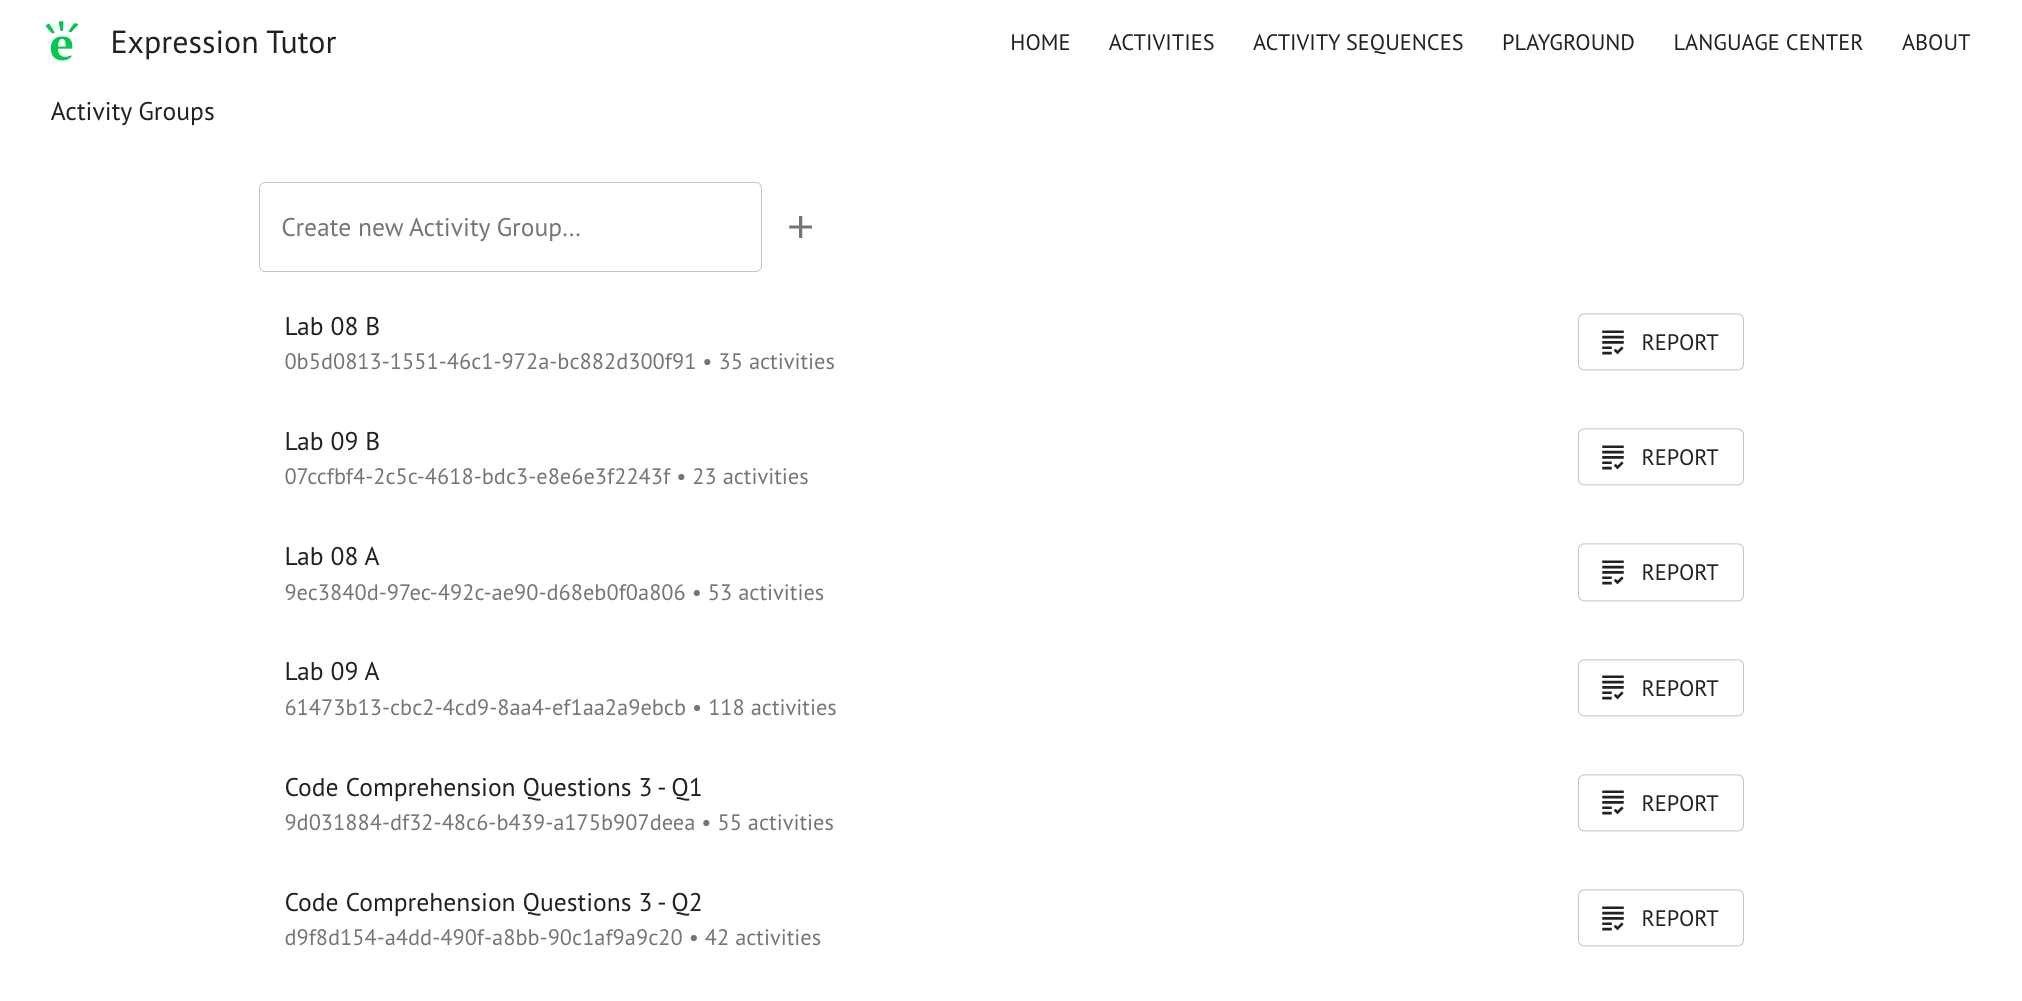
\includegraphics[width=0.8\textwidth]{res/6/ag_list.png}
    \caption{Activity groups overview.}
    \label{fig:impl-ag-list}
\end{figure}

\begin{figure}[ht]
    \centering
    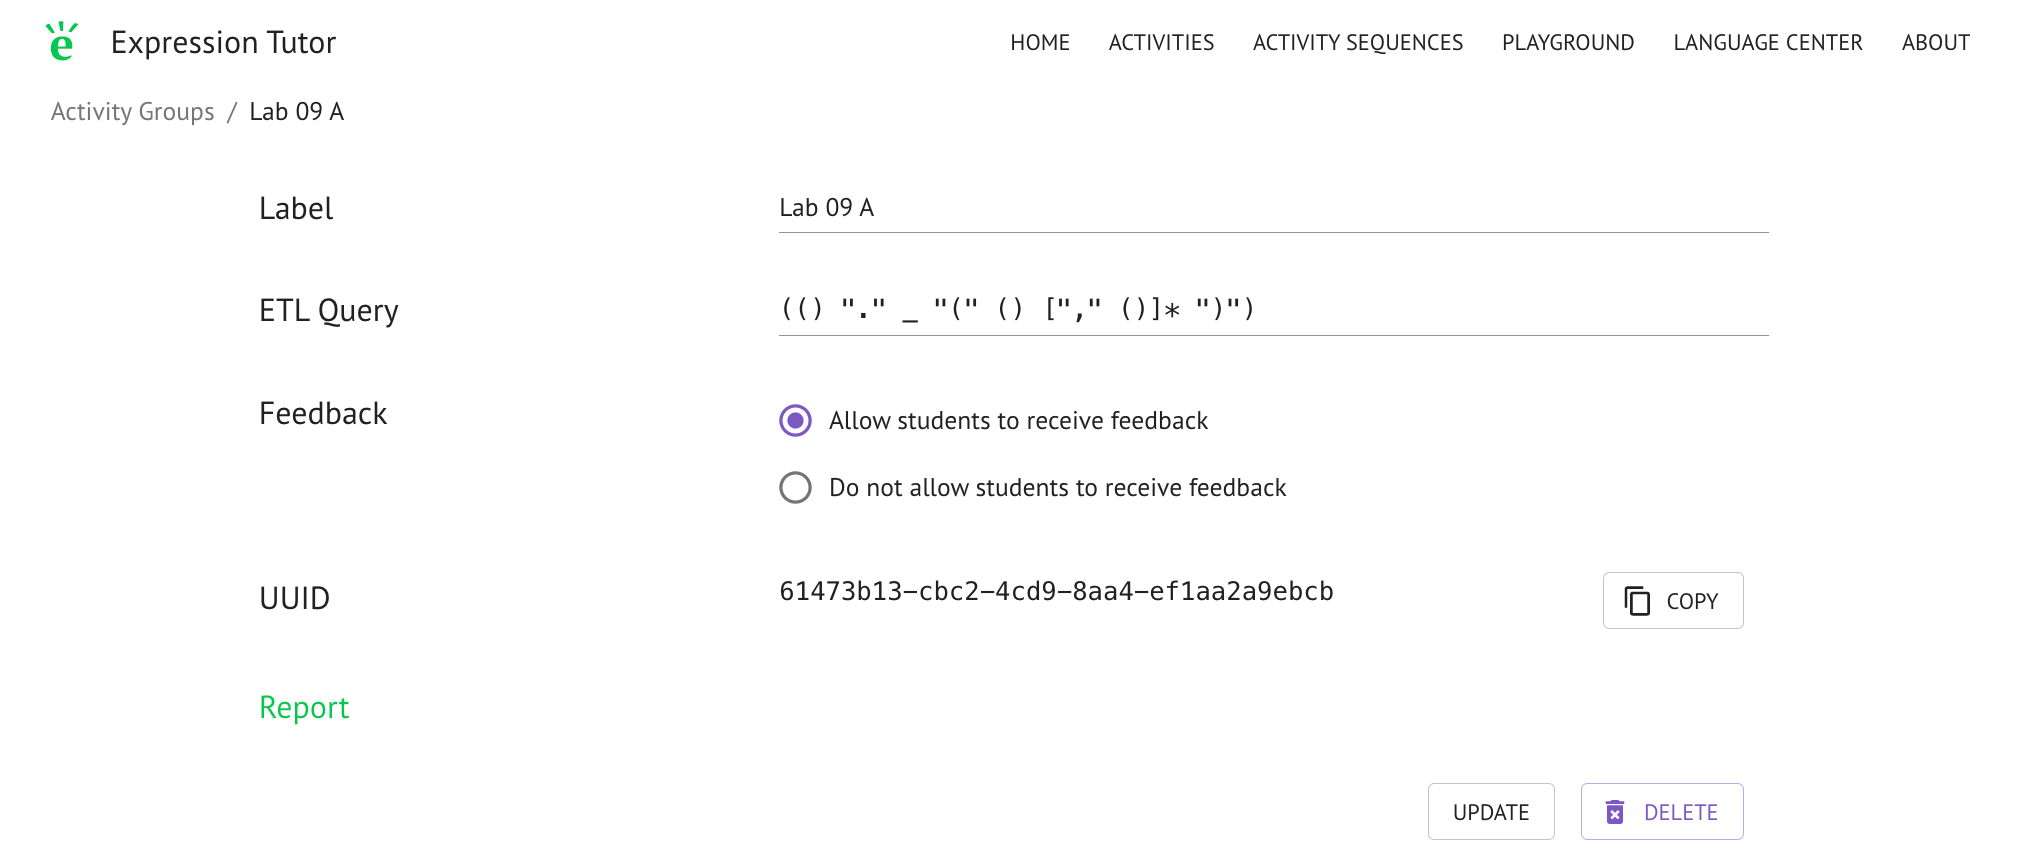
\includegraphics[width=0.8\textwidth]{res/6/ag_details.png}
    \caption{Activity group configuration.}
    \label{fig:impl-ag-details}
\end{figure}

\end{chapterBody}